\tab Ez a modul felelős egy 24 bit-es blokk kiküldéséért. Ehhez a WS2813 egyszálú adatátviteli protokollját be kell, hogy tartsa. 

\tab A legnagyobb kihívás az adott modul megtervezésében a késleltetések implementálása. Ez úgy lett megvalósítva, hogy egy bizonyos állapotban
annyit marad az automata, amíg a megfelelő mennyiségű idő eltelik.


\subsubsection{Elvégzendő RT műveletek azonosítása}

\tab Az időzítések implementálásához egy számláló lesz használva. A 100 MHz-es órajel ami fel lesz használva időben $\SI{0.01}{\micro\second}$-nak felel meg. 
Így a szükséges ciklusok száma (amennyit várakoztatni kell bizonyos feszűltségszinten, ahhoz, hogy a WS2813 protokollja be legyen tartva) egész.
Ebből már látható, hogy definiálható két művelet: $i \Leftarrow ciklus\_szam$, $i \Leftarrow i - 1$ (ahol i a számláló).

\tab Az egyszerűség kedvéért, egy belső regiszternek, amely a színadatokat tartalmazza (\textbf{data}), mindig a 24. bitje kerül kiküldésre.
Tehát minden bit kiküldése után ennek a regiszternek az értékeit el kell csúsztatni (shift-elni) egyet balra: $data \Leftarrow data << 1$

\tab Egy 24-bites blokk kiküldése után kell küldeni egy "RES" jelet, vagyis több ideig alacsony feszűltségen kell tartani a kimenetet. 
Ehhez számolni kell a már elküldött bitek számát $bit\_count \Leftarrow bit\_count - 1$, ahol bit\_count az eddig elküldött bitek számát tartalmazza.
Az elküldött bit-ek 23-től számolódnak lefele, mivel a nullához való hasonlítás hatékonyabb, mint egy adott értékhez való hasonlítás.


\subsubsection{Adatfüggőségek identifikálása}

\tab Mivel nagyon egyszerű RT műveletekkel meg lehet oldani az adott feladatot, nem merűlnek fel adatfüggőségek.


\subsubsection{Célregiszterek azonosítása}

Szükséges regiszterek:
\begin{itemize}
	\item $R_i$: ciklusszámláló regiszter a késleltetésekhez.
	\item $R_{bit\_count}$: Biteket számláló regiszter, a 24 bit-es blokk elküldésének érzékeléséhez.
	\item $R_{data}$: Elküldendő adatot tartalmazó regiszter
\end{itemize}


\subsubsection{Különböző fázisokban elvégzendő műveletek}
\begin{table}[h!]
	\begin{center}
		\caption{WS2813\_Driver - Különböző fázisokban elvégzendő műveletek}
		\begin{tabular}{l|c|c|c|c|c}
		\textbf{Állapot} & $R_i$ 	 & $R_{bit\_count}$     & $R_{data}$      & d\_out 	 & done \\
		\hline         
		READY            & $R_i$ 	 & $R_{bit\_count}$     & $R_{data}$      & 'U' 	 & '0' \\
		\hline         
		INIT          	 & $R_i$ 	 & $24$			        & data      	  & 'U' 	 & $done$ \\
		\hline         
		SEND\_IF01       & $R_i$ 	 & $R_{bit\_count}$     & $R_{data}$      & 'U' 	 & $done$ \\
		\hline         
		SEND1H\_INIT  	 & $T1H$ 	 & $R_{bit\_count}$     & $R_{data}$      & '1' 	 & $done$ \\
		\hline         
		SEND1H           & $R_i - 1$ & $R_{bit\_count}$     & $R_{data}$      & $d\_out$ & $done$ \\
		\hline         
		SEND1L\_INIT     & $T1L$     & $R_{bit\_count}$     & $R_{data}$      & '0'      & $done$ \\
		\hline         
		SEND1L           & $R_i - 1$ & $R_{bit\_count}$     & $R_{data}$      & $d\_out$ & $done$ \\
		\hline         
		SEND0H\_INIT     & $T0H$     & $R_{bit\_count}$     & $R_{data}$      & '1'      & $done$ \\
		\hline         
		SEND0H           & $R_i - 1$ & $R_{bit\_count}$     & $R_{data}$      & $d\_out$ & $done$ \\
		\hline         
		SEND0L\_INIT     & $T0L$     & $R_{bit\_count}$     & $R_{data}$      & '0'      & $done$ \\
		\hline         
		SEND0L           & $R_i - 1$ & $R_{bit\_count}$     & $R_{data}$      & $d\_out$ & $done$ \\
		\hline
		SHIFT\_CHECK     & $R_i$     & $R_{bit\_count} - 1$ & $R_{data}$      & $d\_out$ & $done$ \\
		\hline
		SHIFT	         & $R_i$     & $R_{bit\_count}$     & $R_{data} << 1$ & $d\_out$ & $done$ \\
		\hline
		SENDRES\_INIT    & $TRES$    & $R_{bit\_count}$     & $R_{data}$      & '0'      & $done$ \\
		\hline
		SENDRES          & $R_i - 1$ & $R_{bit\_count}$     & $R_{data}$      & $d\_out$ & $done$ \\
		\hline
		SEND\_DONE       & $R_i$ 	 & $R_{bit\_count}$     & $R_{data}$      & 'U' 	 & '1' \\
		\hline
		DONE\_TODO       & $R_i$ 	 & $R_{bit\_count}$     & $R_{data}$      & 'U' 	 & $done$ \\
		\end{tabular}
	\end{center}
\end{table}


\subsubsection{Kapcsolási rajz}

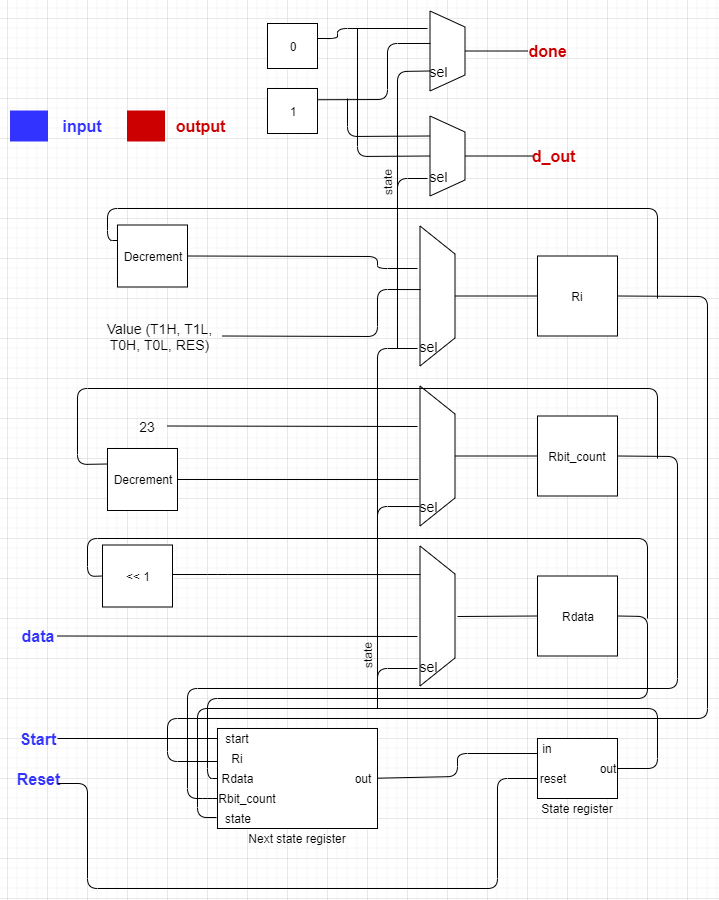
\includegraphics[scale=0.6]{WS2813_Driver_rtl.png}

\subsubsection{Állapotdiagram}

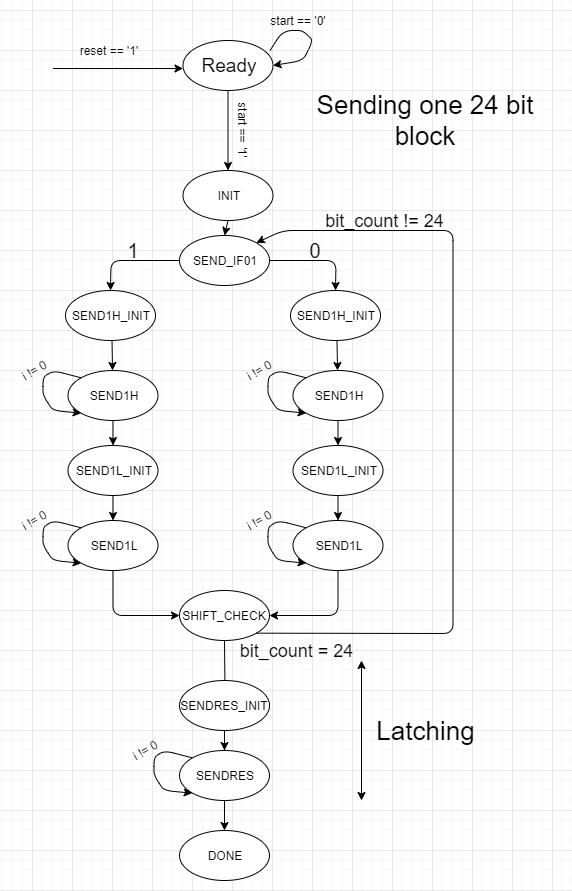
\includegraphics[scale=0.4]{allapotdiagram_final.png}

\begin{itemize}
\item READY
	\begin{itemize}
	\item Alap állapot 
	\item "reset" jel esetén ide kerül vissza az automata
	\end{itemize}
\item INIT
	\begin{itemize}
	\item inicializálja a bit-count-ot nullára
	\end{itemize}
\item SENDIF\_01
	\begin{itemize}
	\item Megvizsgálja data[23]-as bit-et. Ha 1, akkor a következő állapot a \textbf{SEND1H\_INIT}, ha 0 akkor SEND0H\_INIT
	\end{itemize}
\item SEND1H\_INIT
	\begin{itemize}
	\item Inicializálja az \textbf{i} változót a T1H értékre
	\item A d\_out output-ot 1-re állítja
	\end{itemize}
\item SEND1H
	\begin{itemize}
	\item Dekrementálja az \textbf{i} változót
	\item Amikor az \textbf{i} változó nulla lesz, akkor tovább megy a \textbf{SEND1L\_INIT} állapotra
	\end{itemize}
\item SEND1L\_INIT
	\begin{itemize}
	\item Inicializálja az \textbf{i} változót a T1L értékre
	\item A d\_out output-ot 0-ra állítja
	\end{itemize}
\item SEND1L
	\begin{itemize}
	\item Dekrementálja az \textbf{i} változót
	\item Amikor az \textbf{i} változó nulla lesz, akkor tovább megy a \textbf{SHIFT\_CHECK} állapotra
	\end{itemize}
\item SEND0H\_INIT
	\begin{itemize}
	\item Inicializálja az \textbf{i} változót a T0H értékre
	\item A d\_out output-ot 1-re állítja
	\end{itemize}
\item SEND0H
	\begin{itemize}
	\item Dekrementálja az \textbf{i} változót
	\item Amikor az \textbf{i} változó nulla lesz, akkor tovább megy a \textbf{SEND0L\_INIT} állapotra
	\end{itemize}
\item SEND0L\_INIT
	\begin{itemize}
	\item Inicializálja az \textbf{i} változót a T0L értékre
	\item A d\_out output-ot 0-ra állítja
	\end{itemize}
\item SEND0L
	\begin{itemize}
	\item Dekrementálja az \textbf{i} változót
	\item Amikor az \textbf{i} változó nulla lesz, akkor tovább megy a \textbf{SHIFT\_CHECK} állapotra
	\end{itemize}
\item SHIFT\_CHECK
	\begin{itemize}
	\item Megnézi, hogy a \textbf{bit\_count} változó nulla-e, ha igen, akkor tovább megy a \textbf{SENDRES\_INIT} állapotra
	\item Ha a \textbf{bit\_count} változó nem egyenlő nullával, akkor tovább megy a \textbf{SHIFT} állapotra
	\end{itemize}
\item SHIFT
	\begin{itemize}
	\item Shift-eli a \textbf{data} std logic vectort balra eggyel; vissza megy a \textbf{SEND\_IF01} állapotra
	\end{itemize}
\item SENDRES\_INIT
	\begin{itemize}
	\item Inicializálja az \textbf{i} változót a TRES értékre
	\item A d\_out output-ot 0-ra állítja
	\end{itemize}
\item SENDRES
	\begin{itemize}
	\item Dekrementálja az \textbf{i} változót
	\item Amikor az \textbf{i} változó nulla lesz, akkor tovább megy a \textbf{SEND\_DONE} állapotra
	\end{itemize}
\item SEND\_DONE
	\begin{itemize}
	\item Befejeződött a 24 bit-es blokk kiírása
	\item Beállítja a \textbf{done} kimenetet 1-esre
	\end{itemize}
\end{itemize}